\documentclass{article}

\PassOptionsToPackage{numbers, compress}{natbib}
\usepackage[preprint]{neurips_2026}
\usepackage[utf8]{inputenc}
\usepackage[T1]{fontenc}
\usepackage{hyperref}
\usepackage{url}
\usepackage{booktabs}
\usepackage{amsmath}
\usepackage{microtype}
% Status markup, optional blocks and result lookup. The switches are set in status.tex.
\usepackage{etoolbox}\usepackage{array}
\usepackage{xcolor}
\usepackage{graphicx}
\usepackage{pgfplots}
\usetikzlibrary{patterns}
% Chart colors: matplotlib's tab10 order, one fixed color per method; our runs of GG in purple, reported numbers hatched gray
\definecolor{series1}{HTML}{1F77B4}\definecolor{series2}{HTML}{FF7F0E}\definecolor{series3}{HTML}{2CA02C}
\definecolor{series4}{HTML}{D62728}\definecolor{series5}{HTML}{8C564B}
\definecolor{ggours}{HTML}{9467BD}
\pgfplotsset{compat=1.18}

\newbool{submit}
\newtoggle{dsm}             % GRPO (DeepSeekMath) seed 0
\newtoggle{sft}             % SFT on the MBPP-C train problems
\newtoggle{bringupTrained}  % BringUp of the trained checkpoints
\newtoggle{figTrain}        % Figure: training curves
\newtoggle{figDev}          % Figure: dev across checkpoints

% Draft colors; the submitted version prints everything in black.
\newcommand{\statuscolor}[2]{\ifbool{submit}{#2}{\textcolor{#1}{#2}}}
\newcommand{\pending}[1]{\statuscolor{orange}{#1}}  % waits for a run tonight
\newcommand{\todo}[1]{\statuscolor{red}{#1}}        % needs a person: names, wording, a decision
\newcommand{\hand}[1]{\statuscolor{violet}{#1}}     % typed by hand, not yet checked against the result files

% generated/numbers.tex defines \resdef{run/step/metric/stat}{value}. A missing value prints an orange ?? and a
% "Missing result" warning, which ops/report.sh lists and treats as an error in the submitted version.
\newcommand{\resdef}[2]{\csdef{res@#1}{#2}}
\newcommand{\res}[1]{\ifcsdef{res@#1}{\csuse{res@#1}}{\pending{??}\PackageWarning{results}{Missing result #1}}}
\newcommand{\ifres}[3]{\ifcsdef{res@#1}{#2}{#3}}
% \resdash{key}: as \res, but the submitted version prints -- for a missing value (a cell whose eval is still running)
\newcommand{\resdash}[1]{\ifbool{submit}{\ifres{#1}{\res{#1}}{--}}{\res{#1}}}

% \optional{toggle}{key}{content}: shown when the toggle is on. The submitted version also requires a result for key,
% so a row or block whose run did not finish disappears on its own.
\newcommand{\optional}[3]{\iftoggle{#1}{\ifbool{submit}{\ifres{#2}{#3}{}}{#3}}{}}

% Changes against the version approved at 21:35 GST: green background = added, red background
% and struck = deleted. \togglefalse{tracked} prints added text plainly and drops deletions; ops/report.sh refuses a
% submitted build with the marks on.
\usepackage[normalem]{ulem}
\newtoggle{tracked}
\newcommand{\iftracking}[2]{\iftoggle{tracked}{#1}{#2}}
\newcommand{\addedmark}{\bgroup\markoverwith{\textcolor{green!30}{\rule[-0.6ex]{2pt}{2.5ex}}}\ULon}
\newcommand{\deletedmark}{\bgroup\markoverwith{\rlap{\textcolor{red!22}{\rule[-0.6ex]{2pt}{2.5ex}}}%
  \textcolor{red!75!black}{\rule[0.5ex]{2pt}{0.6pt}}}\ULon}
% ulem fails when a hyperlinked citation or reference breaks across lines, so tracked text boxes them whole
\newcommand{\boxlinks}{\let\ULcitep\citep\let\ULcitet\citet\let\ULref\ref
  \renewcommand{\citep}[1]{\mbox{\ULcitep{##1}}}\renewcommand{\citet}[1]{\mbox{\ULcitet{##1}}}\renewcommand{\ref}[1]{\mbox{\ULref{##1}}}}
\DeclareRobustCommand{\added}[1]{\iftracking{\leavevmode{\boxlinks\addedmark{#1}}}{#1}}
\DeclareRobustCommand{\deleted}[1]{\iftracking{\leavevmode{\boxlinks\color{red!60!black}\deletedmark{#1}}}{}}
\DeclareRobustCommand{\addedbox}[1]{\iftracking{\colorbox{green!18}{#1}}{#1}}   % tables, figures, headings
\DeclareRobustCommand{\deletedbox}[1]{\iftracking{\colorbox{red!15}{#1}}{}}   % a removed table: shown on red in the draft only

\newcommand{\draftlegend}{\ifbool{submit}{}{
  \begin{center}\fbox{\parbox{0.92\linewidth}{\small\textbf{Draft.} Black: generated from result files.
  \pending{Orange: waits for a run tonight.} \todo{Red: needs a person.} \hand{Purple: typed by hand, to check.}
  Changes against the 21:35 version: \added{added} \deleted{deleted}. Switches in \texttt{status.tex}.}}\end{center}}}

% Switches. Draft: \boolfalse{submit} shows the status colors and every optional block, with ?? for missing numbers.
% Submitted version: \booltrue{submit}, then turn off any block that is not ready.
\booltrue{submit}
\togglefalse{tracked}   % show changes against the 21:35 version; turn off before submitting

\toggletrue{dsm}   % training ended 19:27 GST; its blocks hide in submit mode until its HumanEval lands
\toggletrue{sft}   % SFT trains between DSM checkpoints (Enzo, Oct 23); its blocks hide in submit mode until HumanEval lands
\toggletrue{bringupTrained}
\toggletrue{figTrain}
\toggletrue{figDev}

\InputIfFileExists{generated/numbers}{}{\PackageWarning{results}{generated/numbers.tex not found}}

\title{Reinforcement Learning with Test Rewards for\\x86-to-ARM Assembly Transpilation\\\large Mid-point Report}

\author{%
  Enzo Shiraishi Nunes da Silva \\
  Mohammed Bin Zayed University of Artificial Intelligence \\
  \texttt{enzo.shiraishi@mbzuai.ac.ae} \\
  \textit{PhD in Computer Science}
  \And
  Sergei Pasynkov \\
  Mohammed Bin Zayed University of Artificial Intelligence \\
  \texttt{sergei.pasynkov@mbzuai.ac.ae} \\
  \textit{PhD in Computer Science}
  \And
  Zayed Khaled Al Tamimi \\
  Mohammed Bin Zayed University of Artificial Intelligence \\
  \texttt{zayed.altamimi@mbzuai.ac.ae} \\
  \textit{PhD in Computer Science}
}

\begin{document}

\maketitle
\draftlegend

\section{Introduction}

Many x86 programs are still in use without their source code, so they cannot simply be recompiled for ARM processors. Dynamic binary translators such as Apple's Rosetta~2 run them anyway, at a cost paid on every execution. A one-time static translation avoids this cost, but only if the translation is correct. Guaranteed Guess (GG) uses a small language model to translate x86 assembly into ARM assembly, and accepts a translation only if it passes the unit tests of the program \citep{gg}. On small benchmark programs, the authors report that the translated code runs 1.73 times faster than the x86 original under Rosetta~2.

GG is trained with supervised fine-tuning (SFT) on pairs of x86 and ARM assembly produced by a compiler, so its loss rewards reproducing the compiler's ARM output token by token. Correctness, however, depends only on behavior, and many different instruction sequences behave identically. The GG authors show correct translations that use other registers, other stack offsets, or a shift and an addition instead of a multiplication, and the SFT loss penalizes each of them. Conversely, a single wrong immediate value changes the behavior of a program but is penalized about as much as a harmless register rename. SFT also trains the model only on reference prefixes, while at generation time it continues from its own output. The weakness is clearest at optimization level O2, where the released model passes 45\% of the HumanEval-C problems, compared with 99\% at O0 \citep{gg}. The unit tests, in contrast, measure behavior directly. They run the translated code on several inputs and execute over 97\% of its lines \citep{gg}. In GG, however, they are used only to accept or reject a translation after it is generated.

We use the tests as a training signal. Starting from the released GG checkpoint for O2, we train the model with Group Relative Policy Optimization (GRPO) \citep{deepseekmath}, where a translation receives a reward of 1 if it passes all tests and 0 otherwise. Any correct translation gets the full reward, and the model learns from its own outputs. GRPO also needs some attempts at a problem to pass and others to fail, which happens at O2 but rarely at O0. Our main research question is whether this training makes the model solve more problems than the released SFT checkpoint. Reinforcement learning with binary rewards mainly raises the probability of solutions the model can already sample \citep{mroueh2025grpo}, so we also ask whether the gains come from problems the baseline solves in some of eight samples, or from problems it never solves.

So far, we have reproduced the baseline with the original compiler toolchain, which regenerates all 328 official HumanEval-C assembly files exactly. Two findings affect any comparison with GG. Library versions alone change the HumanEval-C result of the released model by five problems, or 3 percentage points. The authors' inference script also samples during beam search, while the paper states that sampling was disabled.  Section~\ref{sec:results} reports first results of GRPO and of an SFT baseline trained on the same problems.

Our proposal planned to apply DAPO to vision-language-action (VLA) models \citep{dapo}. We changed the task for three reasons. None of us had used robot simulators before, and each training sample for a VLA is a full simulated episode \citep{simplevlarl,vlarl,rlinfvla}. We have one GPU rather than the two we planned for, which would have allowed too few such episodes. Finally, a simulated task gives one success signal after many actions and depends on the simulator, while a test run gives an exact result for a single generation within seconds. Assembly translation keeps the question of the proposal, reinforcement learning from outcomes after supervised fine-tuning, in a setting where both samples and rewards are cheap.

\section{Related Work}
\label{sec:related}

\paragraph{Reinforcement learning with verifiable rewards.}
Reinforcement learning with verifiable rewards (RLVR) uses a program to check the answer instead of a learned reward model \citep{tulu3}. GRPO suits this setting because it compares several attempts at the same problem and does not require a separate model to predict their results \citep{deepseekmath}. The approach has achieved strong results on verifiable tasks such as mathematics and coding \citep{deepseekr1}, and GRPO with binary rewards has been shown to increase the success probability of the starting model \citep{mroueh2025grpo}.

\paragraph{RLVR for code.}
Code is a natural fit for RLVR because tests give an exact and inexpensive result. RLEF trains code models on the results of running their own code \citep{rlef}, and VeRPO uses partial test results as a denser reward \citep{verpo}. Recent work applies the same idea to low-level code, where the output can be executed or formally verified. SuperCoder uses reinforcement learning to produce faster assembly programs, rewarding both correctness and speed \citep{supercoder}. LLM-VeriOpt trains a small model with GRPO, using a formal verifier as the reward, to optimize compiler code \citep{veriopt}. AutoDecompiler uses compilation and test feedback to train a model that converts binaries back into source code \citep{autodecompiler}, and TRAVEL applies reinforcement learning with execution feedback to translate C code into Rust \citep{travel}. These results show that RLVR can improve code, assembly, and translation. To our knowledge, none applies it to CISC-to-RISC assembly translation.

\paragraph{Assembly translation.}
Guess \& Sketch combines guesses from a language model with a solver that checks whether the translation is equivalent \citep{guesssketch}. CRT is a lightweight language model that translates x86 assembly into ARM and RISC-V \citep{crt}. GG fine-tunes small pre-trained code models (DeepSeek-Coder 1.3B and Qwen2.5-Coder 0.5B and 1.5B) on about 1.3 million C programs from AnghaBench \citep{anghabench} and The Stack v2 \citep{stackv2}, compiled to both instruction sets. It generates candidate translations and checks them with software tests. It is evaluated on HumanEval, a set of programming problems whose C versions are translated and then executed, and on BringupBench, a set of larger programs for embedded systems \citep{gg}. In GG, the tests only filter the model's outputs. We use the same tests as a training signal.

\section{Baseline: the Released GG Model}
\label{sec:baseline}

Our baseline is the released GG checkpoint for ARMv8 at O2, a Qwen2.5-Coder-1.5B-Instruct model \citep{qwen25coder} fine-tuned on the GG data \citep{gg}. We use it without further training. It is also the starting point of our method, so later improvements are measured against it.

\paragraph{Benchmarks and metric.}
HumanEval-C is the C version of HumanEval \citep{humaneval} released with LLM4Decompile \citep{llm4decompile}. It has 164 short functions, each with a test program of assertions. The model receives the x86 assembly of a function, and the assertions decide whether its ARM translation is correct. BringUpBench \citep{bringupbench} is a suite of complete C programs written to bring up new processors and compilers, which depend only on a small bundled library. Its programs are much longer than HumanEval functions, from 85 to 5{,}751 lines \citep{gg}, and a program passes when its output matches the expected output. Following GG, we use the 65 programs that can be built. We report the percentage of problems solved with one prediction per problem, which is the same as pass@1 \citep{humaneval}.

\paragraph{Evaluation harness.}
We implement our own harness so that evaluation and the training reward share the same code. The predicted assembly is the only definition of the function in the test program, which is assembled, linked, and run, so an empty or truncated prediction fails. The GG data targets macOS, so the harness runs on a Mac with Apple Silicon. Data regenerated with a recent Xcode differs from the official files, which were built with Xcode~14.3 and the macOS~13.3 SDK. We therefore built a macOS~13 virtual machine with that toolchain. Inside it, compiling the authors' C code reproduces all 328 official HumanEval-C assembly files exactly. As sanity checks, the reference ARM assembly passes all 164 problems, and an empty prediction fails all of them.

\paragraph{Results.}
Figure~\ref{fig:baseline} gives the results. With beam search, as in the paper, the model solves 77 HumanEval-C problems with the library versions listed with the checkpoint and 72 with newer versions, compared with 74 reported by the authors. Decoding is identical in the two runs, and none of the problems that change reach the length limit, so the gap comes from the library versions alone. A 3-point difference could mask or mimic an improvement of the same size, so we evaluate the baseline and our models with fixed versions. On BringUp, the model solves 6 programs compared with the 10 reported, and the cause is still unknown. We also find that the authors' inference script enables sampling during beam search through the generation configuration of the model, although the paper states that sampling was disabled.  Run as released, it solves 76 problems. 

\begin{table}[h]
\centering
\caption{Environments of our evaluations. Environment~1 has the library versions listed with the released model, and environment~2 is the one we use for training. $^\dagger$PyTorch 2.7 on BringUp, as required by the GPU used for that evaluation.}
\label{tab:software}
\small
%
\begin{tabular}{@{}cll@{}}
\toprule
Environment & Transformers & PyTorch \\
\midrule
1 & 4.50 & 2.6$^\dagger$ \\
2 & 5.17 & 2.13 \\
\bottomrule
\end{tabular}
\end{table}

\begin{table}[h]
\centering
\caption{Our evaluation runs of the released GG model (Figure~\ref{fig:baseline}).}
\label{tab:runs}
\small
%
\begin{tabular}{@{}ccl@{}}
\toprule
Run & Environment & Decoding \\
\midrule
A & 1 & Beam search \\
B & 2 & Beam search \\
C & 1 & Beam search with sampling \\
D & 1 & Greedy \\
\bottomrule
\end{tabular}
\end{table}

\begin{figure}[h]
\centering

%
%
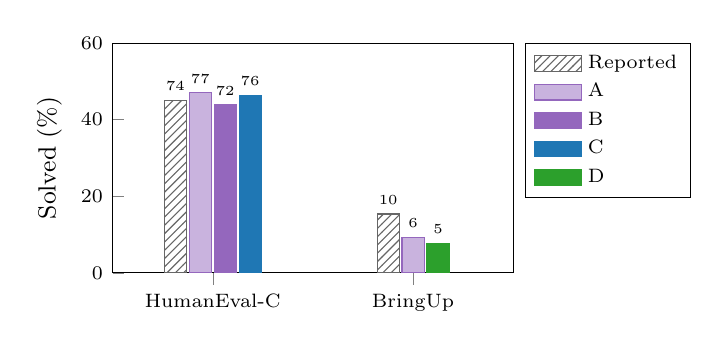
\begin{tikzpicture}\begin{axis}[ybar, bar width=8pt, width=0.55\linewidth, height=4.5cm, ymin=0, ymax=60, ylabel={Solved (\%)},
  symbolic x coords={HumanEval-C,BringUp}, xtick={HumanEval-C,BringUp}, enlarge x limits=0.5, nodes near coords, point meta=explicit symbolic,
  every node near coord/.append style={font=\tiny}, tick label style={font=\scriptsize}, label style={font=\small},
  legend style={font=\scriptsize, cells={anchor=west}}, legend pos=outer north east, area legend, tick pos=left]
\addplot[bar shift=-13.5pt, draw=black!60, pattern=north east lines, pattern color=black!60] coordinates {(HumanEval-C,45.1) [74]}; \addlegendentry{Reported}
\addplot[bar shift=-9pt, draw=black!60, pattern=north east lines, pattern color=black!60, forget plot] coordinates {(BringUp,15.4) [10]};
\addplot[bar shift=-4.5pt, fill=ggours!50, draw=ggours] coordinates {(HumanEval-C,47.0) [77]}; \addlegendentry{A}
\addplot[bar shift=0pt, fill=ggours!50, draw=ggours, forget plot] coordinates {(BringUp,9.2) [6]};
\addplot[bar shift=4.5pt, fill=ggours, draw=ggours] coordinates {(HumanEval-C,43.9) [72]}; \addlegendentry{B}
\addplot[bar shift=13.5pt, fill=series1, draw=series1] coordinates {(HumanEval-C,46.3) [76]}; \addlegendentry{C}
\addplot[bar shift=9pt, fill=series3, draw=series3] coordinates {(BringUp,7.7) [5]}; \addlegendentry{D}
\end{axis}\end{tikzpicture}
\caption{Problems solved by the released GG model at O2. The hatched bars are reported by \citet{gg}. Runs A to D are our evaluations, listed in Table~\ref{tab:runs}, with the number of problems solved above each bar. Beam search uses 8 beams and, as stated by \citet{gg}, no sampling. The released inference code samples during beam search on HumanEval-C and decodes greedily on BringUp. With a limit of 16{,}000 new tokens, run B also gives 72 problems. }
\label{tab:baseline}\label{fig:baseline}
\end{figure}

\section{Proposed Method}
\label{sec:method}

\paragraph{GRPO with a test reward.}
In SFT, the model learns to reproduce a reference translation token by token. GRPO instead learns from its own outputs. It never sees a reference translation, only whether the translations it generates pass the tests. For each training problem, the model samples $G=8$ translations. Translation $i$ gets reward $r_i=1$ if it passes all tests and $r_i=0$ otherwise, and its advantage is
\begin{equation}
  \hat{A}_i = \frac{r_i - \operatorname{mean}(r_1,\dots,r_G)}{\operatorname{std}(r_1,\dots,r_G)},
\end{equation}
applied to every token of the translation \citep{deepseekmath}. The advantage measures how much better translation $i$ is than the average translation of its group. It is positive for a passing translation when some others fail, and negative for a failing one when some others pass. The loss multiplies the log-probability of each token by the advantage of its translation, so an update makes translations with a positive advantage more likely and those with a negative advantage less likely. Passing translations become more likely relative to failing ones, and groups in which all translations pass or all fail do not contribute. In such a group every $r_i$ equals the mean, so every $\hat{A}_i$ is zero (the implementation adds a small constant to the standard deviation, so the division stays defined), and the group does not change the weights. We update all weights of the model. At 1.5 billion parameters, the model, its gradients, and the optimizer states fit on our 96~GB GPU with 32-bit master weights and 16-bit computation, so neither low-rank adapters nor quantization is needed. Because we use no penalty for moving away from the starting model, such as the KL penalty of the original GRPO \citep{deepseekmath}, no separate reference model is kept in memory. The KL divergence measures how much two probability distributions differ. The KL penalty grows as the token probabilities of the trained model move away from those of the reference model, a frozen copy of the starting model, so it keeps the two close. We use the GRPO trainer of TRL \citep{trl} and write the reward function, data preparation, and evaluation ourselves.

\paragraph{Training data.}
MBPP \citep{mbpp} contains short programming problems with assertion tests. We use a C version of it from LLM4Decompile \citep{llm4decompile}, compiled in the same way as the GG data. Of its 973 problems that compile, we keep the 952 whose reference ARM assembly passes its own tests, and split them by distinct x86 program into 858 training and 94 validation problems. HumanEval-C is used only for evaluation. \citet{gg} do not evaluate on MBPP, so no published GG results exist for it. 

\paragraph{Settings.}
Each step uses 16 problems with eight translations each, and training runs for 106 steps, two epochs. Translations are limited to 4{,}096 tokens, which covers the reference of all but 11 training problems, and truncated translations are excluded from the loss. We use the token-level loss of DAPO \citep{dapo} and a learning rate of $10^{-6}$ that decays linearly to zero. The loss of a step is an average over tokens. The original GRPO averages over the tokens of each translation and then over the translations, so a token of a short translation counts more than a token of a long one. The loss of DAPO instead averages over all tokens of the step at once, so every token counts the same. We use gradient accumulation because only 4 translations fit in GPU memory at a time, so each step adds up the gradients of 32 micro-batches of 4 translations. The loss is divided by the number of tokens in the whole step, not in each micro-batch, so the result is the same as if the whole step fit in memory. Unless stated otherwise, GRPO refers to this setup. We evaluate the checkpoint after the last step and do not use the validation set to choose a checkpoint. \optional{dsm}{dsm-seed0/complete}{We also train DeepSeekMath GRPO, the setup of the original paper \citep{deepseekmath}. It averages the loss per translation, keeps truncated translations in the loss, and adds the KL penalty with weight $\beta=0.04$.} \optional{sft}{sft-seed0/complete}{For the SFT baseline, we fine-tune the released model on the reference translations of the same training problems, with the settings of the released GG run (learning rate $2\times10^{-5}$, cosine decay, two epochs) and 16 problems per step as in GRPO. These settings are not tuned.}

\paragraph{Progress and risks.}
 Training runs on a Linux server with one NVIDIA RTX PRO 6000 Blackwell GPU (96~GB), which sends the generated translations through a network tunnel to the Mac and receives the rewards.  Two risks remain. Reward computation on a single Mac limits the training budget. Without a penalty for moving away from the starting model, updating all weights may let the model drift or lose the diversity of its samples, so we will track the entropy of the samples  during training. 


\section{\texorpdfstring{Preliminary Results}{Preliminary Results}}
\label{sec:results}

\subsection{\texorpdfstring{Differences from GG}{Differences from GG}}
\label{sec:differences}
Our setup differs from that of \citet{gg} in the training data, the validation set, the benchmark subsets and the evaluation. The validation set and the two benchmark subsets are ours, so their numbers have no counterpart in that work.

GG is trained with SFT on about 1.3 million programs from AnghaBench \citep{anghabench} and The Stack v2 \citep{stackv2}. We start from the released model and train it further, with GRPO or with SFT for comparison, on 858 MBPP-C problems, which were not used to train or evaluate GG. Of the 865 MBPP-C problems long enough to check, only 25 appear in the GG training data as C code and 76 as assembly, so most of these problems are new to the model.

We hold out 94 MBPP-C problems as a validation set to monitor training (Appendix~\ref{app:dev}). HumanEval-C and BringUp are used only for the final evaluation. We do not use them to choose settings or checkpoints, and we evaluate them only on the final checkpoint of each training run.

We also check for data contamination, that is, benchmark problems that also appear in training data. We find that \res{data/twins} MBPP-C problems are the same as \res{data/twin_problems} HumanEval-C problems, and that \res{data/bringup_contaminated} of the 65 BringUp programs appear in the GG training data. We therefore also check HumanEval-C without these \res{data/twin_problems} problems (Section~\ref{sec:results}). None of the BringUp programs solved by the base model, GRPO or SFT is among these \res{data/bringup_contaminated} programs, so they do not affect the BringUp results.

For decoding, we use beam search with 8 beams and no sampling, as \citet{gg} state, although the released inference script samples during beam search (Section~\ref{sec:baseline}). Library versions change the result on HumanEval-C by up to five problems, so we evaluate all models with the same fixed versions. We use environment~2 of Table~\ref{tab:software} for HumanEval-C and the validation set, and environment~1 for BringUp. We also use our own test harness, with the authors' tests and the original compiler toolchain (Section~\ref{sec:baseline}).

\subsection{\texorpdfstring{Main Results}{Main Results}}

Figure~\ref{fig:main} shows the two benchmarks used by \citet{gg}. GRPO raises the percentage of HumanEval-C problems solved from \res{gg/0/humaneval_beam8/pass1}\% to \res{grpo-seed0/final/humaneval_beam8/pass1}\%. Without the problems that also appear in MBPP-C, it rises from \res{gg/0/humaneval_beam8/clean_pass1}\% to \res{grpo-seed0/final/humaneval_beam8/clean_pass1}\%, so these problems do not explain the gain. Each method is trained with a single seed, so we cannot yet estimate the variance across seeds.

GRPO solves \res{grpo-seed0/final/humaneval_beam8/up} problems that the base model failed and fails \res{grpo-seed0/final/humaneval_beam8/down} that it solved. The base model already solves \res{grpo-seed0/final/humaneval_beam8/upsampled} of these \res{grpo-seed0/final/humaneval_beam8/up} problems in at least one of eight samples at temperature~1, and with more samples it might solve some of the others too.

\optional{sft}{sft-seed0/complete}{Because MBPP-C is new to the model, part of the gain could come from seeing new problems rather than from the reward. The SFT baseline, trained on the same problems, controls for this, and it does not improve HumanEval-C. It solves \res{sft-seed0/final/humaneval_beam8/up} problems that the base model failed and fails \res{sft-seed0/final/humaneval_beam8/down} that it solved. Exposure to new problems therefore does not explain the GRPO gain, at least with this SFT setup. Before SFT, the model already predicts \res{sft-seed0/train/first/accuracy}\% of the tokens of the reference translations, so it has little to learn from them.}

No model changes BringUp by more than two programs. The base model solves \res{gg/0/bringup_beam8/solved} of 65, GRPO solves \res{grpo-seed0/final/bringup_beam8/solved}\optional{sft}{sft-seed0/complete}{, and SFT solves \resdash{sft-seed0/final/bringup_beam8/solved}}. Differences of one or two programs are too small to be conclusive.

\optional{dsm}{dsm-seed0/complete}{DeepSeekMath GRPO solves \res{dsm-seed0/final/humaneval_beam8/up} problems that the base model failed and fails \res{dsm-seed0/final/humaneval_beam8/down} that it solved. \todo{[One sentence comparing the two GRPO setups.]}}

\begin{figure}[h]
\centering
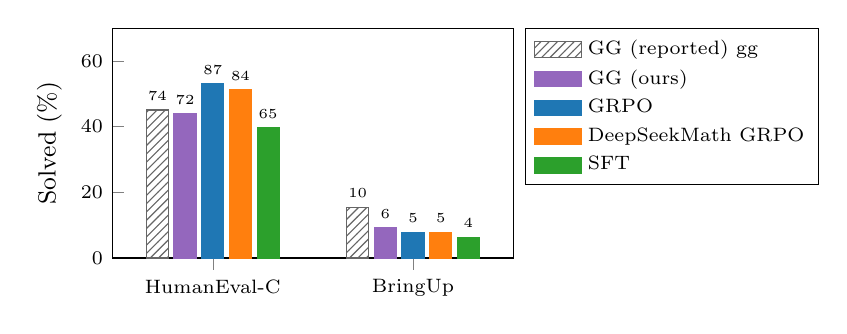
\begin{tikzpicture}\begin{axis}[ybar, bar width=8pt, width=0.55\linewidth, height=4.5cm, ymin=0, ymax=70, ylabel={Solved (\%)}, symbolic x coords={HumanEval-C,BringUp}, xtick=data, tick pos=left, enlarge x limits=0.5, nodes near coords, point meta=explicit symbolic, every node near coord/.append style={font=\tiny}, tick label style={font=\scriptsize}, label style={font=\small}, legend style={font=\scriptsize, cells={anchor=west}}, legend pos=outer north east, area legend]
\addplot[draw=black!60, pattern=north east lines, pattern color=black!60] coordinates {(HumanEval-C,45.1) [74] (BringUp,15.4) [10]};
\addplot[fill=ggours, draw=ggours] coordinates {(HumanEval-C,43.9) [72] (BringUp,9.2) [6]};
\addplot[fill=series1, draw=series1] coordinates {(HumanEval-C,53.0) [87] (BringUp,7.7) [5]};
\addplot[fill=series2, draw=series2] coordinates {(HumanEval-C,51.2) [84] (BringUp,7.7) [5]};
\addplot[fill=series3, draw=series3] coordinates {(HumanEval-C,39.6) [65] (BringUp,6.2) [4]};
\legend{{GG (reported) \citep{gg}},{GG (ours)},{GRPO},{DeepSeekMath GRPO},{SFT}}
\end{axis}\end{tikzpicture}

\caption{Percentage of problems solved with beam search (8 beams) on the two benchmarks used by \citet{gg}, at O2, with the number solved above each bar. The hatched bar is the result reported by \citet{gg}. All other bars are our evaluations, with environment~2 of Table~\ref{tab:software} for HumanEval-C and environment~1 for BringUp. A missing bar marks an evaluation still running.}
\label{fig:main}
\end{figure}

\section{\texorpdfstring{Remaining Work and Task Distribution}{Remaining Work and Task Distribution}}
\label{sec:remaining}

\begin{center}
\small


%
\begin{tabular}{p{0.6\linewidth} p{0.32\linewidth}}
\toprule
\textbf{Goal} & \textbf{Lead} \\
\midrule
Train the GRPO variants, and train each method with three random seeds & Enzo Shiraishi \\
Evaluate other RLVR techniques & Enzo Shiraishi \\
Evaluate the baselines and the trained models on HumanEval-C and BringUp & Zayed Al Tamimi \\
Add training problems with official tests & Sergei Pasynkov \\
Run the ablation with a graded reward & Sergei Pasynkov \\
Run the parameter study on the group size or the learning rate & Zayed Al Tamimi \\
Analyze results and failures, and write the final report & All \\
\bottomrule
\end{tabular}
\end{center}

The final report will compare our method with at least three baselines, namely the released GG model with beam search, the same model with best-of-eight sampling filtered by the tests, and supervised fine-tuning on the reference translations of the same MBPP problems. The ablation will replace the binary reward with a graded one that gives partial credit for assembly that assembles and links, and the parameter study will vary the group size or the learning rate. 

Implementations of GRPO differ in details such as how the loss is averaged, so we will also compare with Dr.~GRPO \citep{drgrpo}, which divides the loss by a constant instead of by the length of each translation and does not divide the advantage by the standard deviation\ifres{dsm-seed0/complete}{}{, and with DeepSeekMath GRPO \citep{deepseekmath}, which adds the KL penalty}. We will train every method with three random seeds and tune the hyperparameters of SFT.

In \res{grpo-seed0/train/all/zerostd}\% of the groups during GRPO training, all eight translations pass or all fail, so they give no gradient (Appendix~\ref{app:training}), and MBPP-C has only 858 training problems. We will add problems only from sources with official judge tests, which gives 890 Codeforces problems \citep{codeforces} and up to 1{,}832 AOJ problems \citep{codenet}, about 2.5 times the size of MBPP-C. These problems are judged on their printed output, so the reward needs an output-comparison mode.

We also want to try other RLVR methods for the groups that give no gradient, such as the dynamic sampling of DAPO, which only keeps groups with both passing and failing translations \citep{dapo}, or larger groups. We also plan to compare with rejection-sampling fine-tuning, which trains the model on its own passing translations \citep{star,raft}.

We will sample the base model more than eight times on the problems that GRPO gains, look for the reason why we solve 6 BringUp programs compared with the 10 reported, and study why GRPO solves more problems with beam search on HumanEval-C but not on the validation set.

{\small
\bibliographystyle{plainnat}
\bibliography{references}
}

\appendix

\section{\texorpdfstring{Training}{Training}}
\label{app:training}
At every step, the model samples 8 translations for each of 16 training problems, and the reward server tests them. Figure~\ref{fig:training} shows two quantities, averaged over 10 steps. The pass rate is the fraction of the 128 translations of a step that pass all tests. It averages \res{grpo-seed0/train/e1/reward}\% in the first epoch and \res{grpo-seed0/train/e2/reward}\% in the second, so the model improves slightly on its training problems. A group gives no gradient when all eight translations pass or all fail. In that case every reward equals the mean of the group, every advantage in Equation~(1) is zero, and the group does not change the weights. This happens in \res{grpo-seed0/train/all/zerostd}\% of the groups, so more than half of the problems of a step do not contribute to it.

\optional{figTrain}{grpo-seed0/train/hours}{%
\begin{figure}[h]
\centering
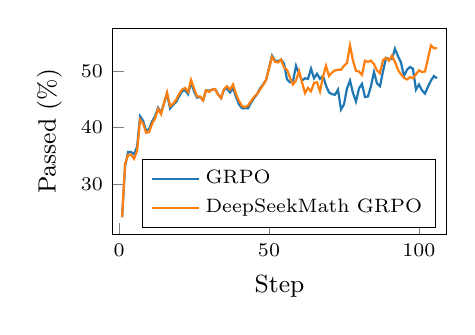
\begin{tikzpicture}\begin{axis}[width=0.48\linewidth, height=4.2cm, xlabel=Step, enlarge x limits=0.03, tick pos=left, tick label style={font=\scriptsize}, label style={font=\small}, legend style={font=\scriptsize, cells={anchor=west}}, ylabel={Passed (\%)}, legend pos=south east]
\addplot[series1, thick] coordinates {(1,24.2) (2,33.2) (3,35.7) (4,35.7) (5,35.3) (6,36.6) (7,42.0) (8,41.2) (9,39.5) (10,39.7) (11,41.1) (12,42.0) (13,43.5) (14,42.6) (15,44.3) (16,46.0) (17,43.4) (18,44.0) (19,44.5) (20,45.5) (21,46.4) (22,46.6) (23,45.9) (24,48.0) (25,46.4) (26,45.3) (27,45.4) (28,44.8) (29,46.6) (30,46.5) (31,46.7) (32,46.8) (33,45.9) (34,45.2) (35,46.7) (36,46.9) (37,46.2) (38,47.0) (39,45.4) (40,44.1) (41,43.4) (42,43.4) (43,43.4) (44,44.4) (45,45.2) (46,45.9) (47,46.9) (48,47.6) (49,48.4) (50,50.5) (51,52.7) (52,51.8) (53,51.7) (54,52.0) (55,51.3) (56,48.5) (57,48.0) (58,48.2) (59,50.9) (60,49.5) (61,48.3) (62,48.7) (63,48.6) (64,50.4) (65,48.7) (66,49.5) (67,48.6) (68,49.1) (69,47.4) (70,46.2) (71,45.9) (72,45.8) (73,46.7) (74,43.2) (75,44.1) (76,46.9) (77,48.3) (78,46.1) (79,44.6) (80,46.9) (81,47.7) (82,45.4) (83,45.5) (84,47.3) (85,49.8) (86,47.8) (87,47.3) (88,49.9) (89,52.3) (90,52.1) (91,52.1) (92,53.9) (93,52.6) (94,51.5) (95,49.1) (96,50.2) (97,50.7) (98,50.4) (99,46.7) (100,47.6) (101,46.6) (102,46.0) (103,47.2) (104,48.3) (105,49.1) (106,48.7)};
\addplot[series2, thick] coordinates {(1,24.2) (2,33.6) (3,35.2) (4,35.2) (5,34.5) (6,35.9) (7,41.4) (8,40.7) (9,39.1) (10,39.2) (11,40.7) (12,41.6) (13,43.3) (14,42.4) (15,44.4) (16,46.2) (17,43.8) (18,44.2) (19,44.9) (20,45.9) (21,46.7) (22,47.0) (23,46.3) (24,48.4) (25,46.9) (26,45.5) (27,45.5) (28,44.8) (29,46.6) (30,46.3) (31,46.7) (32,46.8) (33,45.8) (34,45.2) (35,46.8) (36,47.3) (37,46.7) (38,47.6) (39,45.9) (40,44.7) (41,43.8) (42,43.6) (43,43.9) (44,44.7) (45,45.4) (46,45.9) (47,46.7) (48,47.5) (49,48.4) (50,50.4) (51,52.5) (52,51.6) (53,51.5) (54,52.0) (55,50.6) (56,50.2) (57,48.8) (58,47.6) (59,48.3) (60,50.0) (61,48.0) (62,46.1) (63,47.0) (64,46.4) (65,47.9) (66,48.0) (67,46.4) (68,49.0) (69,50.9) (70,49.1) (71,49.7) (72,50.1) (73,50.2) (74,50.2) (75,50.9) (76,51.4) (77,54.5) (78,51.8) (79,50.0) (80,49.9) (81,49.3) (82,51.8) (83,51.6) (84,51.8) (85,51.2) (86,50.1) (87,49.6) (88,51.9) (89,52.3) (90,51.8) (91,52.7) (92,51.6) (93,50.2) (94,49.4) (95,48.8) (96,48.5) (97,48.9) (98,48.7) (99,49.4) (100,50.1) (101,49.8) (102,49.9) (103,52.2) (104,54.5) (105,54.0) (106,54.0)};
\legend{{GRPO},{DeepSeekMath GRPO}}
\end{axis}\end{tikzpicture}\hfill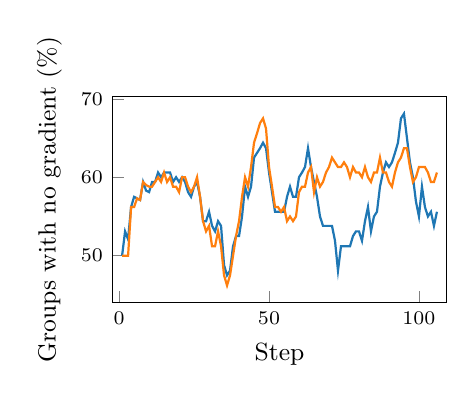
\begin{tikzpicture}\begin{axis}[width=0.48\linewidth, height=4.2cm, xlabel=Step, enlarge x limits=0.03, tick pos=left, tick label style={font=\scriptsize}, label style={font=\small}, legend style={font=\scriptsize, cells={anchor=west}}, ylabel={Groups with no gradient (\%)}]
\addplot[series1, thick] coordinates {(1,50.0) (2,53.1) (3,52.1) (4,56.2) (5,57.5) (6,57.3) (7,57.1) (8,59.4) (9,58.3) (10,58.1) (11,59.4) (12,59.4) (13,60.6) (14,60.0) (15,60.6) (16,60.6) (17,60.6) (18,59.4) (19,60.0) (20,59.4) (21,60.0) (22,59.4) (23,58.1) (24,57.5) (25,58.8) (26,59.4) (27,57.5) (28,54.4) (29,54.4) (30,55.6) (31,53.8) (32,53.1) (33,54.4) (34,53.8) (35,48.8) (36,47.5) (37,48.1) (38,51.2) (39,52.5) (40,52.5) (41,55.0) (42,58.8) (43,57.5) (44,58.8) (45,62.5) (46,63.1) (47,63.7) (48,64.4) (49,63.7) (50,60.6) (51,58.1) (52,55.6) (53,55.6) (54,55.6) (55,55.6) (56,57.5) (57,58.8) (58,57.5) (59,57.5) (60,60.0) (61,60.6) (62,61.3) (63,63.7) (64,61.3) (65,59.4) (66,57.5) (67,55.0) (68,53.8) (69,53.8) (70,53.8) (71,53.8) (72,51.9) (73,48.1) (74,51.2) (75,51.2) (76,51.2) (77,51.2) (78,52.5) (79,53.1) (80,53.1) (81,51.9) (82,54.4) (83,56.2) (84,53.1) (85,55.0) (86,55.6) (87,58.8) (88,60.6) (89,61.9) (90,61.3) (91,61.9) (92,63.1) (93,64.4) (94,67.5) (95,68.1) (96,65.0) (97,61.9) (98,60.0) (99,56.9) (100,55.0) (101,58.8) (102,56.2) (103,55.0) (104,55.6) (105,53.8) (106,55.6)};
\addplot[series2, thick] coordinates {(1,50.0) (2,50.0) (3,50.0) (4,56.2) (5,56.2) (6,57.3) (7,57.1) (8,59.4) (9,59.0) (10,58.8) (11,58.8) (12,59.4) (13,60.0) (14,59.4) (15,60.6) (16,59.4) (17,60.0) (18,58.8) (19,58.8) (20,58.1) (21,60.0) (22,60.0) (23,58.8) (24,58.1) (25,58.8) (26,60.0) (27,57.5) (28,54.4) (29,53.1) (30,53.8) (31,51.2) (32,51.2) (33,53.1) (34,51.2) (35,47.5) (36,46.2) (37,47.5) (38,50.0) (39,52.5) (40,54.4) (41,57.5) (42,60.0) (43,58.8) (44,61.3) (45,64.4) (46,65.6) (47,66.9) (48,67.5) (49,66.2) (50,61.3) (51,58.8) (52,56.2) (53,56.2) (54,55.6) (55,56.2) (56,54.4) (57,55.0) (58,54.4) (59,55.0) (60,58.1) (61,58.8) (62,58.8) (63,60.6) (64,61.3) (65,58.1) (66,60.0) (67,58.8) (68,59.4) (69,60.6) (70,61.3) (71,62.5) (72,61.9) (73,61.3) (74,61.3) (75,61.9) (76,61.3) (77,60.0) (78,61.3) (79,60.6) (80,60.6) (81,60.0) (82,61.3) (83,60.0) (84,59.4) (85,60.6) (86,60.6) (87,62.5) (88,60.6) (89,60.6) (90,59.4) (91,58.8) (92,60.6) (93,61.9) (94,62.5) (95,63.7) (96,63.7) (97,61.3) (98,59.4) (99,60.0) (100,61.3) (101,61.3) (102,61.3) (103,60.6) (104,59.4) (105,59.4) (106,60.6)};
\end{axis}\end{tikzpicture}

\caption{Training curves, averaged over 10 steps. Left: pass rate of the 128 translations of a step. Right: groups in which all eight translations pass or all fail, which give no gradient.}
\label{fig:training}
\end{figure}}

\optional{sft}{sft-seed0/complete}{For SFT, Figure~\ref{fig:sft} shows the loss on the reference translations and the share of their tokens that the model predicts correctly. The token accuracy is already \res{sft-seed0/train/first/accuracy}\% at the first step and ends at \res{sft-seed0/train/last/accuracy}\%, so the released model already reproduces the reference translations almost exactly. The loss rises during the first epoch, while the learning rate is highest, and falls during the second, from \res{sft-seed0/train/first/loss} at the first step to \res{sft-seed0/train/last/loss} at the last. The drop of the validation pass rate after the first epoch (Appendix~\ref{app:dev}) coincides with this rise.

\begin{figure}[h]
\centering
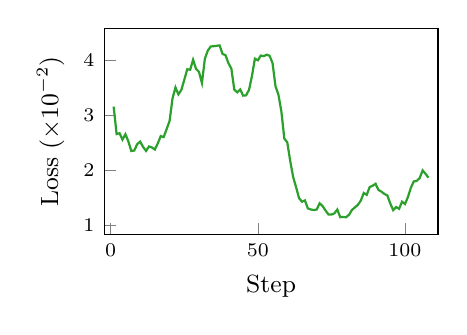
\begin{tikzpicture}\begin{axis}[width=0.48\linewidth, height=4.2cm, xlabel=Step, enlarge x limits=0.03, tick pos=left, tick label style={font=\scriptsize}, label style={font=\small}, legend style={font=\scriptsize, cells={anchor=west}}, ylabel={Loss ($\times 10^{-2}$)}]
\addplot[series3, thick] coordinates {(1,3.152) (2,2.655) (3,2.67) (4,2.554) (5,2.652) (6,2.52) (7,2.347) (8,2.356) (9,2.472) (10,2.517) (11,2.422) (12,2.349) (13,2.43) (14,2.411) (15,2.374) (16,2.486) (17,2.618) (18,2.6) (19,2.744) (20,2.891) (21,3.3) (22,3.5) (23,3.375) (24,3.456) (25,3.639) (26,3.829) (27,3.822) (28,4.003) (29,3.838) (30,3.781) (31,3.582) (32,4.023) (33,4.17) (34,4.244) (35,4.248) (36,4.256) (37,4.263) (38,4.11) (39,4.085) (40,3.941) (41,3.842) (42,3.46) (43,3.411) (44,3.464) (45,3.352) (46,3.357) (47,3.457) (48,3.709) (49,4.022) (50,3.993) (51,4.079) (52,4.068) (53,4.095) (54,4.074) (55,3.941) (56,3.521) (57,3.368) (58,3.063) (59,2.571) (60,2.504) (61,2.166) (62,1.875) (63,1.69) (64,1.492) (65,1.428) (66,1.45) (67,1.305) (68,1.287) (69,1.276) (70,1.286) (71,1.399) (72,1.349) (73,1.267) (74,1.196) (75,1.194) (76,1.216) (77,1.285) (78,1.147) (79,1.149) (80,1.146) (81,1.191) (82,1.279) (83,1.325) (84,1.37) (85,1.449) (86,1.586) (87,1.552) (88,1.693) (89,1.717) (90,1.752) (91,1.641) (92,1.61) (93,1.568) (94,1.542) (95,1.395) (96,1.274) (97,1.331) (98,1.298) (99,1.427) (100,1.385) (101,1.512) (102,1.679) (103,1.796) (104,1.805) (105,1.857) (106,1.995) (107,1.933) (108,1.863)};
\end{axis}\end{tikzpicture}\hfill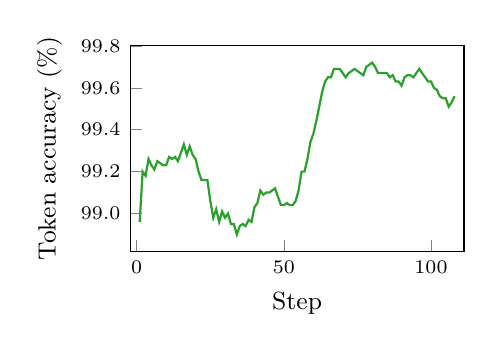
\begin{tikzpicture}\begin{axis}[width=0.48\linewidth, height=4.2cm, xlabel=Step, enlarge x limits=0.03, tick pos=left, tick label style={font=\scriptsize}, label style={font=\small}, legend style={font=\scriptsize, cells={anchor=west}}, ylabel={Token accuracy (\%)}, yticklabel style={/pgf/number format/.cd, fixed, fixed zerofill, precision=1}]
\addplot[series3, thick] coordinates {(1,98.96) (2,99.2) (3,99.18) (4,99.26) (5,99.23) (6,99.21) (7,99.25) (8,99.24) (9,99.23) (10,99.23) (11,99.27) (12,99.26) (13,99.27) (14,99.25) (15,99.29) (16,99.33) (17,99.28) (18,99.32) (19,99.28) (20,99.26) (21,99.2) (22,99.16) (23,99.16) (24,99.16) (25,99.06) (26,98.98) (27,99.02) (28,98.96) (29,99.01) (30,98.98) (31,99) (32,98.95) (33,98.95) (34,98.9) (35,98.94) (36,98.95) (37,98.94) (38,98.97) (39,98.96) (40,99.03) (41,99.05) (42,99.11) (43,99.09) (44,99.1) (45,99.1) (46,99.11) (47,99.12) (48,99.08) (49,99.04) (50,99.04) (51,99.05) (52,99.04) (53,99.04) (54,99.06) (55,99.11) (56,99.2) (57,99.2) (58,99.26) (59,99.34) (60,99.38) (61,99.44) (62,99.51) (63,99.58) (64,99.63) (65,99.65) (66,99.65) (67,99.69) (68,99.69) (69,99.69) (70,99.67) (71,99.65) (72,99.67) (73,99.68) (74,99.69) (75,99.68) (76,99.67) (77,99.66) (78,99.7) (79,99.71) (80,99.72) (81,99.7) (82,99.67) (83,99.67) (84,99.67) (85,99.67) (86,99.65) (87,99.66) (88,99.63) (89,99.63) (90,99.61) (91,99.65) (92,99.66) (93,99.66) (94,99.65) (95,99.67) (96,99.69) (97,99.67) (98,99.65) (99,99.63) (100,99.63) (101,99.6) (102,99.59) (103,99.56) (104,99.55) (105,99.55) (106,99.51) (107,99.53) (108,99.56)};
\end{axis}\end{tikzpicture}

\caption{Training of SFT, averaged over 10 steps. Left: loss on the reference translations. Right: share of the reference tokens predicted correctly.}
\label{fig:sft}
\end{figure}}

\section{\texorpdfstring{Validation Set}{Validation Set}}
\label{app:dev}
The validation set has 94 MBPP-C problems held out from training, from the same source as the training data. We use it only to monitor training, not to choose a checkpoint. We report the percentage of problems solved with beam search, as for the benchmarks, and with sampling at temperature~1, averaged over 8 samples per problem (Figure~\ref{fig:dev}). With beam search, the base model solves \res{gg/0/dev_beam8/pass1}\% of the problems and GRPO \res{grpo-seed0/final/dev_beam8/pass1}\%\optional{sft}{sft-seed0/complete}{, and SFT \res{sft-seed0/final/dev_beam8/pass1}\%}, so the result with beam search is essentially unchanged, unlike on HumanEval-C. With sampling, GRPO goes from \res{gg/0/dev_sample8/pass1}\% to \res{grpo-seed0/final/dev_sample8/pass1}\%.\optional{sft}{sft-seed0/complete}{ SFT drops to \res{sft-seed0/54/dev_sample8/pass1}\% after its first epoch and ends at \res{sft-seed0/final/dev_sample8/pass1}\%. Of its \res{sft-seed0/final/dev_sample8/samples} samples, \res{sft-seed0/final/dev_sample8/asmerr} fail to assemble, compared with \res{gg/0/dev_sample8/asmerr} for the base model and \res{grpo-seed0/final/dev_sample8/asmerr} after GRPO.}

\optional{figDev}{grpo-seed0/final/dev_sample8/pass1}{%
\begin{figure}[h]
\centering
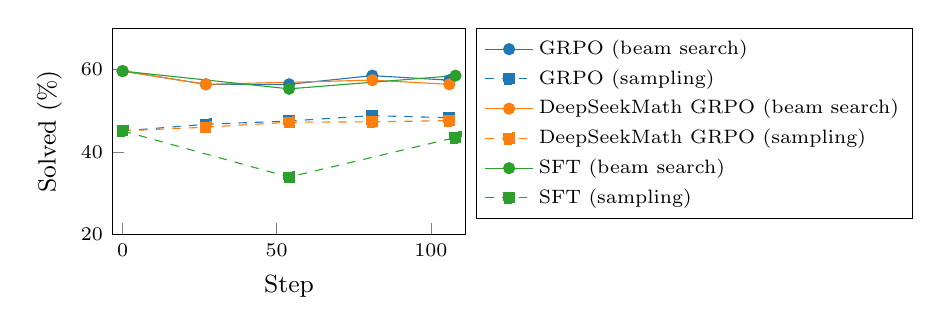
\begin{tikzpicture}\begin{axis}[width=0.5\linewidth, height=4.2cm, xlabel=Step, enlarge x limits=0.03, tick pos=left, tick label style={font=\scriptsize}, label style={font=\small}, legend style={font=\scriptsize, cells={anchor=west}}, ylabel={Solved (\%)}, ymin=20, ymax=70, legend pos=outer north east]
\addplot[series1, mark=*] coordinates {(0,59.6) (27,56.4) (54,56.4) (81,58.5) (106,57.4)};
\addlegendentry{GRPO (beam search)}
\addplot[series1, mark=square*, dashed] coordinates {(0,45.1) (27,46.7) (54,47.5) (81,48.8) (106,48.3)};
\addlegendentry{GRPO (sampling)}
\addplot[series2, mark=*] coordinates {(0,59.6) (27,56.4) (81,57.4) (106,56.4)};
\addlegendentry{DeepSeekMath GRPO (beam search)}
\addplot[series2, mark=square*, dashed] coordinates {(0,45.1) (27,46.0) (54,47.2) (81,47.3) (106,47.6)};
\addlegendentry{DeepSeekMath GRPO (sampling)}
\addplot[series3, mark=*] coordinates {(0,59.6) (54,55.3) (108,58.5)};
\addlegendentry{SFT (beam search)}
\addplot[series3, mark=square*, dashed] coordinates {(0,45.1) (54,33.9) (108,43.5)};
\addlegendentry{SFT (sampling)}
\end{axis}\end{tikzpicture}

\caption{Percentage of the 94 validation problems solved at each checkpoint, with beam search (solid) and with sampling at temperature~1 (dashed). Step 0 is the base model.}
\label{fig:dev}
\end{figure}}

\end{document}